\documentclass[../../main.tex]{subfiles}
\graphicspath{{\subfix{../../image/}}} % 指定图片目录,后续可以直接使用图片文件名。

% 例如:
% \begin{figure}[H]
% \centering
% \includegraphics[scale=0.4]{图.png}
% \caption{}
% \label{figure:图}
% \end{figure}
% 注意:上述\label{}一定要放在\caption{}之后,否则引用图片序号会只会显示??.

\begin{document}

\section{有限群}

\begin{definition}[有限群]
设$(G,\cdot)$ 是一个群.我们称 $G$ 是一个\textbf{有限群},若 $G$ 是有限的。 
\end{definition}

\begin{definition}[元素的阶]
设$(G,\cdot)$ 是一个群,若 $x\in G$,则 $x$(在 $G$ 中)的\textbf{阶},记作 $|x|$,定义为那个最小的正整数 $n\in\mathbb{N}_1$,使得 $x^n = e$。若这样的 $n$ 不存在,则记 $|x|=\infty$。 
\end{definition}

\begin{proposition}[有限群的每个元素的阶必有限]\label{proposition:有限群的每个元素的阶必有限}
若 $(G,\cdot)$ 是有限群,且 $x\in G$,则 $|x|<\infty$。换言之,有限群的每一个元素通过自乘有限多次,都可以得到单位元。
\end{proposition}
\begin{proof}
我们用反证法,假设 $|x|=\infty$,那么根据定义,对于任意的 $n\in\mathbb{N}_1$,我们都有 $x^n\neq e$。我们要说明的是,这会导致一个事实,就是所有的 $x^n(n\in\mathbb{N}_1)$ 都是不同的。假设但凡有一对 $n\neq m\in\mathbb{N}_1$ 使得 $x^n = x^m$,不失一般性我们假设 $n>m$。则通过反复的消元(两边反复右乘$x^{-1}$),我们可以得到 $x^{n - m}=e$,其中 $n - m\in\mathbb{N}_1$,而这与假设是矛盾的,因为我们假设 $x$ 的阶是无穷的。因此,这个事实是对的——所有的 $x^n(n\in\mathbb{N}_1)$ 都是不同的,从而$G$中有无穷多个元素,这与$G$是有限群矛盾.这就证明了这个命题。 
\end{proof}

\begin{proposition}\label{proposition:关于幂的群同态}
设 $(G,\cdot)$ 是一个群,任取 $x\in G$。则
\begin{align*}
f:(\mathbb{Z} ,+)&\rightarrow (G,\cdot )
\\
n&\mapsto x^n
\end{align*}
是一个群同态。
\end{proposition}
\begin{proof}
取定 $x\in G$。令 $m,n\in\mathbb{Z}$,我们只须证明 $f(m + n)=f(m)\cdot f(n)$,也即 $x^{m + n}=x^m\cdot x^n$。于是根据\hyperref[proposition:关于元素幂的一些性质]{命题\ref{proposition:关于元素幂的一些性质}(1)}就能立即得到结论.
\end{proof}

\begin{definition}[由 $x$ 生成的群]
设 $(G,\cdot)$ 是一个群,且 $x\in G$,则 $\langle x\rangle$,被称为\textbf{由 $x$ 生成的群},定义为
\begin{align*}
\langle x\rangle=\{x^n:n\in\mathbb{Z}\}.
\end{align*} 
\end{definition}

\begin{proposition}\label{proposition:<x>是一个子群}
设 $(G,\cdot)$ 是一个群,且 $x\in G$,则 $\langle x\rangle<G$.
\end{proposition}
\begin{proof}
记
\begin{align*}
f:(\mathbb{Z} ,+)&\rightarrow (G,\cdot )
\\
n&\mapsto x^n
\end{align*}
由\hyperref[proposition:关于幂的群同态]{命题\ref{proposition:关于幂的群同态}}可知$f$是一个群同态.注意到 $\mathrm{im}\,f=\langle x\rangle$,即$\langle x \rangle$是$f$的同态像.从而由\hyperref[proposition:群同态的核是定义域的子群,像是陪域的子群]{命题\ref{proposition:群同态的核是定义域的子群,像是陪域的子群}}可知,$\langle x\rangle=\mathrm{im}\,f<G$.
\end{proof}

\begin{definition}[由 $S$ 生成的群]
设 $(G,\cdot)$ 是一个群,且 $S\subset G$。则\textbf{由 $S$ 生成的群},记作 $\langle S\rangle$,定义为
\begin{align*}
\langle S\rangle=\bigcap\{H\subset G:H\supset S, H < G\}
\end{align*}
\end{definition}

\begin{proposition}
令 $(G,\cdot)$ 是一个群,且 $S\subset G$,则 $\langle S\rangle < G$.
\end{proposition}
\begin{note}
这个命题表明:$G$ 中由 $S$ 生成的子群,确实是包含了 $S$ 的最小子群.
\end{note}
\begin{proof}
在这里,我们只要证明其包含单位元,在乘法和逆元下封闭。

根据定义,$\langle S\rangle$ 是由所有包含了 $S$ 的 $G$ 中子群全部取交集得到的。

单位元:每个这样的子群 $H$ 都包含单位元,故它们的交集也包含单位元。

乘法封闭性:设 $x,y\in\langle S\rangle$,任取一个包含了 $S$ 的子群 $H$,则 $x,y\in H$。因为 $H$ 是子群,故 $xy\in H$,所以由$H$的任意性可知$xy\in\langle S\rangle$。

逆元封闭性:设$x\in \langle S\rangle$,任取一个包含了 $S$ 的子群 $H$,则 $x\in H$。因为 $H$ 是子群,故 $x^{-1}\in H$,所以由$H$的任意性可知$x^{-1}\in\langle S\rangle$.
\end{proof}

\begin{definition}[循环群]
令 $(G,\cdot)$ 是一个群。若存在 $x\in G$,使得 $G = \langle x\rangle=\left\{ x^n:n\in \mathbb{Z} \right\} $,则 $G$ 被称为一个\textbf{循环群},而 $x$ 被称为 $G$ 的一个\textbf{生成元}.

若$G$还是一个有限群,则我们称$G$为\textbf{有限循环群}.若$G$不是有限群,则我们称$G$为\textbf{无限循环群}.
\end{definition}
\begin{remark}
我们一般用$C_n$表示$n$阶循环群.
\end{remark}
\begin{note}
有限循环群与无限循环群示意图如下:
\begin{figure}[H]
\centering
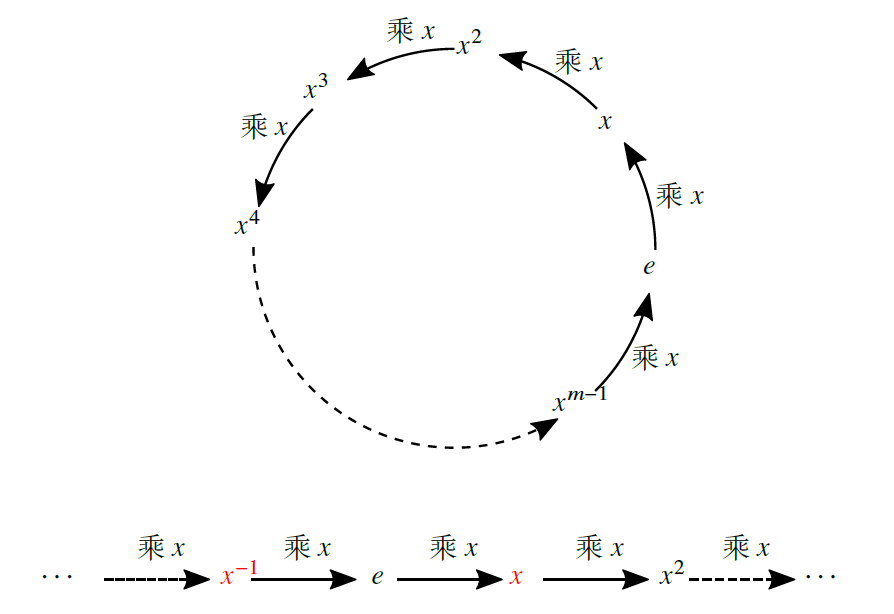
\includegraphics[scale=0.4]{有限循环群和无线循环群.png}
\label{figure:有限循环群和无线循环群}
\caption{有限循环群和无线循环群}
\end{figure}
\end{note}

\begin{proposition}\label{proposition:由x生成的群就是由子集{x}生成的子群}
设 $(G,\cdot)$ 是一个群,对$\forall x\in G$,都有 $\langle x\rangle=\langle\{x\}\rangle$.
\end{proposition}
\begin{note}
这个命题表明:由$x$生成的群就是由子集$\{x\}$生成的子群.
\end{note}
\begin{proof}
根据定义和性质,$\langle\{x\}\rangle$ 是包含了 $\{x\}$ 的最小的子群。因此要证明这个最小的子群就是 $\langle x\rangle$,我们只须证明两点。一,$\langle x\rangle$ 是个子群;二,如果一个子群 $H$ 包含了 $\{x\}$,那么它一定要包含整个 $\langle x\rangle$。

首先,由\hyperref[proposition:<x>是一个子群]{命题\ref{proposition:<x>是一个子群}}可知$\langle x\rangle$ 是个子群。这就证明了第一点。

第二点几乎也是显然的。我们设 $H$ 是个子群,且 $x\in H$。那么根据子群包含单位元,且有乘法和逆元的封闭性,我们有 $e\in H$,并且递归地,对于 $\forall n\in\mathbb{N}_1$,都有$x^n = x\cdots x\in H$,$x^{-n}=x^{-1}\cdots x^{-1}\in H$。这就证明了 $H\supset\langle x\rangle$。 
\end{proof}

\begin{proposition}\label{proposition:有限循环群的元素可用枚举法全部列举出来}
设 $G = \langle x\rangle$ 是有限循环群,并且 $|x| = n$,则 $G=\{e,x,x^2,\cdots,x^{n - 1}\}$,并且$\{e,x,x^2,\cdots,x^{n - 1}\}$中的这些元素是两两不同的。我们称这样的有限循环群的阶是 $n$。
\end{proposition}
\begin{proof}
我们来证明两件事。第一,每一个 $G$ 中   元素都可以写成从 $0$ 开始的前 $n$ 项幂的形式;第二,从 $0$ 开始的前 $n$ 项幂是两两不同的。

我们来证明第一点。任取 $G$ 中元素 $x^m$,其中 $m\in\mathbb{Z}$。根据带余除法,存在$q\in\mathbb{Z}$,$0\leqslant  r\leqslant  n - 1$,使得 $m = qn + r$.那么因为 $x^n = e$,所以 $x^m = x^{qn + r}=(x^n)^q\cdot x^r = x^r$,而这就属于从 $0$ 开始的前 $n$ 项幂。

我们来证明第二点。用反证法,假设 $0\leqslant  m' < m\leqslant  n - 1$,使得 $x^m = x^{m'}$,则 $x^{m - m'} = e$。其中 $1\leqslant  m - m'\leqslant  n - 1 < n$,可是 $n = |x|$ 是最小的正整数 $k$ 使 $x^k = e$,这就导致了矛盾。

综上所述,$G=\{e,x,x^2,\cdots,x^{n - 1}\}$,其中枚举法中的这些元素是两两不同的。 
\end{proof}

\begin{proposition}\label{proposition:所有有限阶循环群彼此同构}
对于任意的 $n\in\mathbb{N}_1$,所有 $n$ 阶的循环群都是互相同构的.
\end{proposition}
\begin{proof}
设 $G = \langle x\rangle, G' = \langle y\rangle$ 都是 $n$ 阶循环群。令
\begin{align*}
f:G\rightarrow G'
,
x^m\mapsto y^m
\end{align*}
则对$\forall x^{m_1},x^{m_2}\in G$,其中$1\leqslant  m_1,m_2\leqslant  n-1$.我们都有
\begin{align*}
f\left( x^{m_1}x^{m_2} \right) =f\left( x^{m_1+m_2} \right) =y^{m_1+m_2}=y^{m_1}y^{m_2}=f\left( x^{m_1} \right) f\left( x^{m_2} \right) .
\end{align*}
因此$f$是个同态映射.
此外,它是个双射,因为我们可以明确地找到其逆映射
\begin{align*}
f^{-1}(y^m)&=x^m
\end{align*}
这样,$f$ 既是双射,也是同态,这就证明了 $f$ 是个同构。 
\end{proof}

\begin{proposition}\label{proposition:每一个无限循环群都对应两个生成元}
设$G = \langle x\rangle$ 是无限循环群,则 $x^n(n\in\mathbb{Z})$ 是两两不同的,且 $G$ 只有两个生成元,分别是 $x$ 与 $x^{-1}$。
\end{proposition}
\begin{note}
显然,$(\mathbb{Z},+)$就是一个无限循环群,生成元是1或-1.
\end{note}
\begin{proof}
首先证明 $x^n(n\in\mathbb{Z})$ 是两两不同的。假设有两个相同,不失一般性假设 $m > n\in\mathbb{Z},x^m = x^n$,则 $x^{m - n}=e$,故 $x$ 是有有限阶的。这就矛盾了。

接着,如果 $x^n(n\in\mathbb{Z})$ 可以生成这个群,那么 $x\in\langle x^n\rangle$,于是存在 $m\in\mathbb{Z}$ 使得 $x=(x^n)^m$,于是 $x^{nm - 1}=e$。由于 $x$ 是无限阶的,所以 $nm = 1$,那么这样的 $n$ 只能是 $\pm1$。另外,显然 $x^{-1}$ 也可以生成这个群。这就证明了恰好是这两个生成元。
\end{proof}

\begin{proposition}\label{proposition:所有的无限循环群是彼此同构的}
所有的无限循环群是彼此同构的.进而所有的无限循环群$\langle x\rangle(|x|=\infty)$都同构于整数加群$(\mathbb{Z},+)$.
\end{proposition}
\begin{note}
这个命题告诉我们:要研究无限循环群,只要研究整数加群$(\mathbb{Z},+)$就可以了.
\end{note}
\begin{proof}
设 $G = \langle x\rangle, G' = \langle y\rangle$ 都是 无限循环群。令
\begin{align*}
f:G\rightarrow G'
,
x^m\mapsto y^m
\end{align*}
则对$\forall x^{m_1},x^{m_2}\in G$,其中$m_1,m_2\in \mathbb{Z}$.我们都有
\begin{align*}
f\left( x^{m_1}x^{m_2} \right) =f\left( x^{m_1+m_2} \right) =y^{m_1+m_2}=y^{m_1}y^{m_2}=f\left( x^{m_1} \right) f\left( x^{m_2} \right) .
\end{align*}
因此$f$是个同态映射.
此外,它是个双射,因为我们可以明确地找到其逆映射
\begin{align*}
f^{-1}(y^m)&=x^m
\end{align*}
这样,$f$ 既是双射,也是同态,这就证明了 $f$ 是个同构。
\end{proof}

\begin{proposition}\label{proposition:有限循环群的阶的计算公式}
令 $G = \langle x\rangle$ 是一个 $n$ 阶循环群。假设 $1\leqslant  m\leqslant  n$,则 $x^m$ 的阶为
\begin{align*}
|x^m|=\frac{n}{\gcd(n,m)}.
\end{align*}
\end{proposition}
\begin{proof}
设 $1\leqslant  m\leqslant  n - 1$,我们希望找到最小的正整数 $k$ 使得 $(x^m)^k = x^{mk}=e$。由于 $|x| = n$,故这等价于 $n\mid mk$。接下来我们要利用简单的初等数论。通过同时除以 $n$ 和 $m$ 的最大公因数,我们得到
\begin{align*}
\frac{n}{\gcd(n,m)}\Bigg|\frac{m}{\gcd(n,m)}\cdot k
\end{align*}
而因为 $\frac{n}{\gcd(n,m)}$ 和 $\frac{m}{\gcd(n,m)}$ 是互素的,所以这个条件进一步等价于
\begin{align*}
\frac{n}{\gcd(n,m)}\Bigg|k
\end{align*}
也就是说,最小的这个正整数 $k$ 正是 $\frac{n}{\gcd(n,m)}$。这就完成了证明.
\end{proof}

\begin{proposition}\label{proposition:有限循环群的生成元的充要条件}
令 $G = \langle x\rangle$ 是一个 $n$ 阶循环群,则 $x^m(1\leqslant  m\leqslant  n)$ 是个生成元,当且仅当
\begin{align*}
\gcd(m,n)=1.
\end{align*}
根据欧拉 $\phi$ 函数的定义,这些生成元的个数正是 $\phi(n)$。 
\end{proposition}
\begin{proof}
若$x^m$是一个生成元,则由$G$是一个$n$阶循环群可知,$|x^m|=n$.从而由\hyperref[proposition:有限循环群的阶的计算公式]{命题\ref{proposition:有限循环群的阶的计算公式}}可知,$\gcd(m,n)=\frac{n}{|x^m|}=1$.

若$\gcd(m,n)=1$,则由\hyperref[proposition:有限循环群的阶的计算公式]{命题\ref{proposition:有限循环群的阶的计算公式}}可知,$|x^m|=\frac{n}{\gcd(n,m)}=n$.从而
\begin{align*}
\left( x^m \right) ^n=e,\,\left( x^m \right) ^{n+1}=\left( x^m \right) ^nx=x,\cdots ,\left( x^m \right) ^{2n-1}=\left( x^m \right) ^nx^{n-1}=x^{n-1}.
\end{align*}
又由\hyperref[proposition:有限循环群的元素可用枚举法全部列举出来]{命题\ref{proposition:有限循环群的元素可用枚举法全部列举出来}}可知$G=\{e,x,\cdots,x^{n-1}\}$.于是
\begin{align*}
G=\left\{ e,x,\cdots ,x^{n-1} \right\} =\left\{ \left( x^m \right) ^n,\left( x^m \right) ^{n+1},\cdots ,\left( x^m \right) ^{2n-1} \right\}=\left\{ \left( x^m \right) ^n:n\in \mathbb{Z} \right\} .
\end{align*}
因此$G=\langle x^m\rangle$,故$x^m$是$G$的生成元.
\end{proof}

\begin{definition}[群的阶]
设$(G,\cdot)$是一个群,则$G$的阶,记作$|G|$,定义为$G$的集合大小(元素的个数).
\end{definition}

\begin{definition}[子群的阶]
设$(G,\cdot)$是一个群,$H$是$G$的子群,则$H$的阶,记作$|H|$,定义为$H$的集合大小(元素的个数)。若$H$是无限群则记$|H| = \infty$。
\end{definition}

\begin{definition}[左陪集]
设$G$是一个群,$H < G$是一个子群,$a \in G$。则称$aH$是$H$的一个(由$a$引出的)\textbf{左陪集},定义为
\begin{align*}
aH = \{ax : x \in H\}.
\end{align*}
称$aH$是$H$的一个(由$a$引出的)\textbf{右陪集},定义为
\begin{align*}
Ha = \{xa : x \in H\}.
\end{align*} 
\end{definition}
\begin{remark}
$aH,Ha$一般来说不是$G$的子群.

我们只讨论左陪集的性质和结论,右陪集的性质与左陪集类似.
\end{remark}

\begin{lemma}\label{lemma:陪集aH大小与H相同}
令$G$是一个有限群,$H < G$是一个子群,$a \in G$。令
\begin{align*}
f : H \to aH,x \mapsto ax.
\end{align*}
则$f$是一个双射。特别地,$|H| = |aH|$。 
\end{lemma}
\begin{note}
这个引理表明:陪集的大小都是一样的.
\end{note}
\begin{proof}
{\color{blue}证法一:}
根据$f$的定义易知$f$是满射.若 \(f(h_1) = f(h_2)\),则
\begin{align*}
ah_1 = ah_2 &\Rightarrow a^{-1}ah_1 = a^{-1}ah_2 \Rightarrow h_1 = h_2.
\end{align*}
故 \(f\) 也是单射。因此 \(f\) 是双射。

{\color{blue}证法二:}
令
\[g: aH \rightarrow H, k \mapsto a^{-1}k.\]
设 \(k \in aH\),则存在 \(h \in H\),使得 \(k = ah\)。则 \(g(k) = g(ah) = a^{-1}ah = h \in H\)。故 \(g\) 是良定义的。
注意到
\begin{align*}
g \circ f = \mathrm{id}_H, \quad f \circ g = \mathrm{id}_{aH}.
\end{align*}
故 \(g\) 是 \(f\) 的逆映射。因此 \(f\) 是双射。 
\end{proof}

\begin{proposition}\label{proposition:两个左陪集要么相等要么无交}
设$G$是一个有限群,$H < G$是一个子群,$a,b \in G$。则左陪集$aH$和$bH$要么相等,要么无交。也就是说,我们有$aH = bH$,或$aH \cap bH = \emptyset$。
\end{proposition}
\begin{proof}
假设$aH\cap bH \neq \emptyset$,则可设$ah_1 = bh_2 \in aH\cap bH$,其中$h_1,h_2 \in H$。我们只须证明$aH = bH$,而根据对称性,我们只须证明$aH \subset bH$即可。任取$aH$中的元素$ah (h \in H)$,则由$ah_1 = bh_2$可知,$a=bh_2h_1^{-1}$.从而
\begin{align*}
ah=(bh_2h_1^{-1})h = b(h_2h_1^{-1}h) \in bH
\end{align*}
这就完成了证明.
\end{proof}

\begin{definition}[商集]\label{definition:商集和其指数}
设\(G\) 是一个非空集合,\(H \subset G\) 是一个子集合.则\textbf{商集} \(G/H\) 定义为
\begin{align*}
G/H = \{aH : a \in G\}.
\end{align*}
\textbf{商集} \(H\backslash G\) 定义为
\begin{align*}
H\backslash G = \{Ha : a \in G\}.
\end{align*}
我们把商集\(G/H\)的大小(所含元素的个数)称为 \(H\) 在 \(G\) 中的\textbf{指数},记为 \([G : H]\),即
\begin{align*}
[G : H] = |G/H|.
\end{align*} 
\end{definition}

\begin{theorem}\label{theorem:商集G/H构成G的一个分拆}
设$G$是一个有限群,$H < G$是一个子群,则商集 \(G/H= \{aH : a \in G\}\)就是$G$的一个分拆,即
\[
G=\bigsqcup_{i=1}^{\left[ G:H \right]}{a_iH}=\bigsqcup_{a\in G}{aH}.
\]
\end{theorem}
\begin{proof}
一方面,设 \(x \in G\),取 \(a = x\),则 \(x = xe = ae \in xH\).
另一方面,由由\hyperref[proposition:两个左陪集要么相等要么无交]{命题\ref{proposition:两个左陪集要么相等要么无交}}可知,对 \(\forall aH, bH \in G/H\),都有 \(aH\) 和 \(bH\) 要么相等,要么无交.故商集 \(G/H= \{aH : a \in G\}\)就是$G$的一个分拆.
\end{proof}
\begin{note}
\begin{figure}[H]
\centering
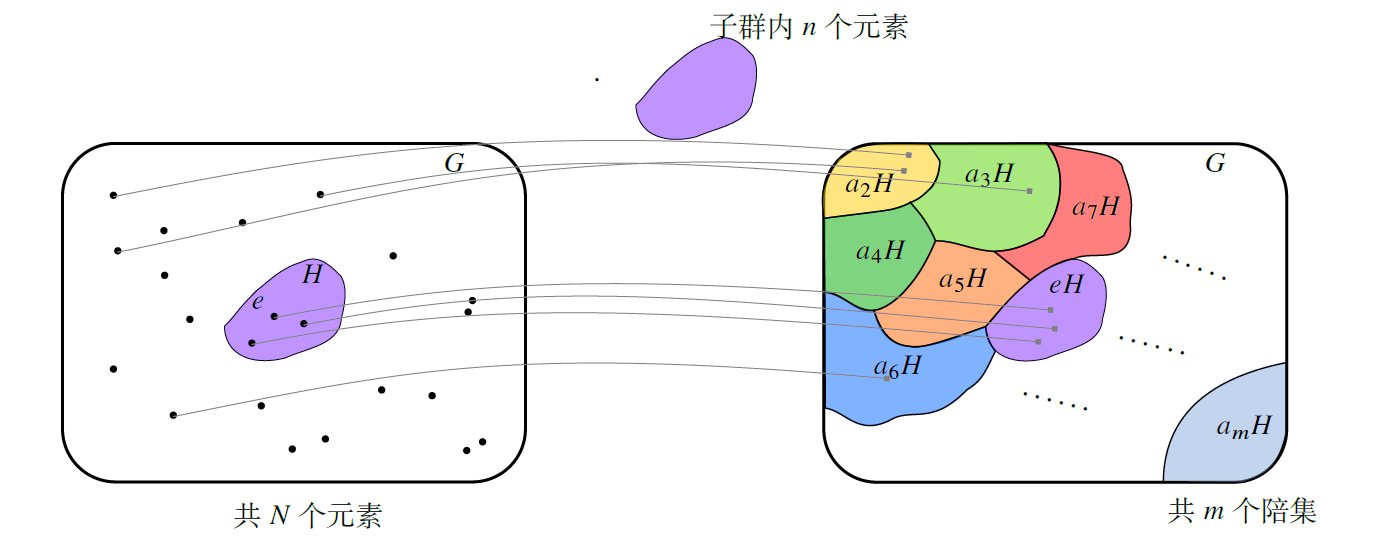
\includegraphics[scale=0.4]{左陪集示意图.png}
\label{figure:左陪集示意图}
\caption{左陪集示意图}
\end{figure}
\end{note}

\begin{theorem}[Lagrange定理]\label{theorem:Lagrange定理}
设\(G\) 是一个有限群,\(H < G\) 是一个子群,则
\begin{align*}
|G| = [G : H]|H|.
\end{align*}
进而$[G : H]=\frac{|G|}{|H|}$.
特别地,
\begin{align*}
|H| \Big| |G|.
\end{align*} 
\end{theorem}
\begin{proof}
由\hyperref[theorem:商集G/H构成G的一个分拆]{定理\ref{theorem:商集G/H构成G的一个分拆}}可知$G=\bigsqcup_{i=1}^{\left[ G:H \right]}{a_iH},$从而
\[
\left| G \right|=\sum_{i=1}^{\left[ G:H \right]}{\left|a_iH_i\right|}.
\]
又由\hyperref[lemma:陪集aH大小与H相同]{引理\ref{lemma:陪集aH大小与H相同}}可知$\left|a_iH_i\right|=\left|H\right|$.故\begin{align*}
|G| = [G : H]|H|.
\end{align*}
\end{proof}

\begin{example}
设 $(G,\cdot)$ 是一个群,若 $|G| = p$ 是素数,则不存在任何非平凡子群.
\end{example}
\begin{proof}
设 $H < G$,则由\hyperref[theorem:Lagrange定理]{Lagrange 定理}可知 $|H|\mid |G|$,即 $|H|\mid p$。从而 $|H| = 1$ 或 $p$,于是 $H = \{e\}$ 或 $G$。 
\end{proof}

\begin{lemma}\label{lemma:两个相等的陪集同时左乘相同元素保持等号}
设 \(G\) 是一个群,\(H < G\) 是一个子群,$x,y,a,b\in G$,则
\begin{enumerate}[(1)]
\item $xH \subset yH \Leftrightarrow axHb \subset ayHb.$

\item $Hx\subset Hy \Leftrightarrow aHxb\subset aHyb.$


\item $xH\subset Hy \Leftrightarrow axHb\subset aHyb.$
\end{enumerate}
进一步,我们有
\begin{enumerate}[(1)]\setcounter{enumi}{3}
\item $xH=yH \Leftrightarrow axHb=ayHb.$

\item $Hx=Hy \Leftrightarrow aHxb=aHyb.$


\item $xH=Hy \Leftrightarrow axHb=aHyb.$
\end{enumerate}
\end{lemma}
\begin{proof}
\begin{enumerate}[(1)]\setcounter{enumi}{3}
\item $\Rightarrow:$若 \(xH = yH\),则要证 \(axHb = ayHb\),根据对称性,只须证 \(axHb \subset ayHb\)。任取 \(axhb \in axHb\),其中 \(h \in H\),则由 \(xH = yH\) 及 \(xh \in xH\) 可知,存在 \(h' \in H\),使得 \(xh = yh'\)。从而 \(axhb = ayh'b \in ayHb\)。故 \(axHb \subset ayHb\)。

$\Leftarrow:$若 \(axHb = ayHb\),则要证 \(xH = yH\),根据对称性,只须证 \(xH \subset yH\)。任取 \(xh \in xH\),其中 \(h \in H\),则由 \(axHb = ayHb\) 及 \(axhb \in axHb\) 可知,存在 \(h' \in H\),使得 \(axhb = ayh'b\)。从而 \(xh = a^{-1}axhbb^{-1} = a^{-1}ayh'bb^{-1} = yh' \in yH\)。故 \(xH \subset yH\).

\item $\Rightarrow:$若 \(Hx = Hy\),则要证 \(aHxb = aHyb\),根据对称性,只须证 \(aHxb \subset aHyb\).任取 \(ahxb \in aHxb\),其中 \(h \in H\),则由 \(Hx = Hy\) 及 \(hx \in Hx\) 可知,存在 \(h' \in H\),使得 \(hx = h'y\)。从而 \(ahxb = ah'yb \in aHyb\)。故 \(aHxb \subset aHyb\)。

$\Leftarrow:$若 \(aHbx = aHyb\),则要证 \(Hx = Hy\),根据对称性,只须证 \(Hx \subset Hy\)。任取 \(hx \in Hx\),其中 \(h \in H\),则由 \(aHxb = aHyb\) 及 \(ahxb \in aHxb\) 可知,存在 \(h' \in H\),使得 \(ahxb = ah'yb\)。从而 \(hx = a^{-1}ahxbb^{-1} = a^{-1}ah'ybb^{-1} = h'y \in Hy\)。故 \(Hx \subset Hy\).

\item $\Rightarrow:$若 \(xH = Hy\),则要证 \(axHb = aHyb\),根据对称性,只须证 \(axHb \subset aHyb\)。任取 \(axhb \in axHb\),其中 \(h \in H\),则由 \(xH = Hy\) 及 \(xh \in xH\) 可知,存在 \(h' \in H\),使得 \(xh = h'y\)。从而 \(axhb = ah'yb \in aHyb\)。故 \(axHb \subset aHyb\)。

$\Leftarrow:$若 \(axHb = aHyb\),则要证 \(xH = Hy\),根据对称性,只须证 \(xH \subset Hy\)。任取 \(xh \in xH\),其中 \(h \in H\),则由 \(axHb = aHyb\) 及 \(axhb \in axHb\) 可知,存在 \(h' \in H\),使得 \(axhb = ah'yb\)。从而 \(xh = a^{-1}axhbb^{-1} = a^{-1}ah'ybb^{-1} = h'y \in Hy\)。故 \(xH \subset Hy\).
\end{enumerate}

根据上述(4)(5)(6)的证明过程就能直接得到(1)(2)(3)的证明.
\end{proof}

\begin{lemma}\label{lemma:关于两个陪集相等的充要条件}
设 \(G\) 是一个群,\(H < G\) 是一个子群,\(x \in G\),则我们有充要条件
\begin{align*}
xH = H \iff x \in H .
\end{align*}
一般地,对于 \(x, y \in G\),我们有充要条件
\begin{align*}
xH = yH \iff y^{-1}x \in H \iff x^{-1}y \in H \iff x\in yH \iff y\in xH.
\end{align*}
\end{lemma}
\begin{note}
同理可知对右陪集也有相同的结论.
\end{note}
\begin{proof}
对于$x\in G$,
一方面,设 \(xH = H\),则\(x = xe \in xH = H\),因此 \(x \in H\)。

另一方面,{\color{blue}证法一:}设 \(x \in H\),任取 \(xh \in xH\),则根据乘法封闭性可知 \(xh \in H\)。故 \(xH \subset H\)。
任取 \(h \in H\),则根据乘法封闭性和逆元封闭性可知 \(x^{-1}h \in H\),从而 \(h = xx^{-1}h \in xH\)。 故 \(H \subset xH\).因此$xH=H$.

{\color{blue}证法二:}设 \(x \in H\),则$x=xe\in xH$.从而$xH \cap H\ne \emptyset$.于是由\hyperref[proposition:两个左陪集要么相等要么无交]{命题\ref{proposition:两个左陪集要么相等要么无交}}可知$xH=H$.

综上,我们就有$xH = H \iff x \in H .$

一般地,对于$x,y\in G$,
由\hyperref[lemma:两个相等的陪集同时左乘相同元素保持等号]{引理\ref{lemma:两个相等的陪集同时左乘相同元素保持等号}}可知\(xH=yH\Leftrightarrow y^{-1}xH=H\Leftrightarrow H=x^{-1}yH,\)又由上述证明可知
\begin{align*}
y^{-1}xH=H\Longleftrightarrow y^{-1}x\in H,x^{-1}yH=H\Longleftrightarrow x^{-1}y\in H.
\end{align*}
故$xH = yH \iff y^{-1}x \in H \iff x^{-1}y \in H.$
下证$xH=yH \iff x\in yH \iff y\in xH.$

一方面,设 \(xH = yH\),则\(x = xe \in xH = yH\),因此 \(x \in yH\)。
另一方面,设 \(x \in yH\),则$x=xe\in xH$.从而$xH \cap yH\ne \emptyset$.于是由\hyperref[proposition:两个左陪集要么相等要么无交]{命题\ref{proposition:两个左陪集要么相等要么无交}}可知$xH=yH$.故$xH=yH \iff x\in yH$.同理可证$xH=yH \iff y\in xH$.
\end{proof}

\begin{corollary}\label{corollary:关于两个陪集相等的充要条件推论}
\begin{enumerate}[(1)]
\item 设 \(G\) 是一个群,\(H < G\) 是一个子群,\(a \in G\),则
\begin{align*}
axH=aH \iff x\in H.
\end{align*}

\item 设 \(G\) 是一个群,$K<H<G$,$a_1,a_2\in G,b_1,b_2 \in H$.若$a_1b_1K=a_2b_2K$,则$a_1H=a_2H$.
\end{enumerate}
\end{corollary}
\begin{note}
同理可知对右陪集也有相同的结论.
\end{note}
\begin{proof}
\begin{enumerate}[(1)]
\item 由\hyperref[lemma:两个相等的陪集同时左乘相同元素保持等号]{引理\ref{lemma:两个相等的陪集同时左乘相同元素保持等号}}可知\[axH=aH \iff xH=H.\]
又由\hyperref[lemma:关于两个陪集相等的充要条件]{引理\ref{lemma:关于两个陪集相等的充要条件}}可知\[xH=H \iff x\in H.\]故\[axH=aH \iff x\in H.\]

\item 由\hyperref[lemma:关于两个陪集相等的充要条件]{引理\ref{lemma:关于两个陪集相等的充要条件}}可知$b_{2}^{-1}a_{2}^{-1}a_1b_1\in K$,从而存在$k\in K$,使得$b_{2}^{-1}a_{2}^{-1}a_1b_1=k$,于是$a_2^{-1}a_1=b_2kb_{1}^{-1}\in H.$再根据\hyperref[lemma:关于两个陪集相等的充要条件]{引理\ref{lemma:关于两个陪集相等的充要条件}}可知$a_1H=a_2H.$
\end{enumerate}
\end{proof}

\begin{proposition}
令 \(K < H < G\) 是三个有限群,则
\begin{align*}
[G : K] = [G : H][H : K] .
\end{align*}
\end{proposition}
\begin{proof}
{\color{blue}证法一:}由\hyperref[theorem:Lagrange定理]{Lagrange定理}可得
\begin{align*}
\left[ G:K \right] =\frac{\left| G \right|}{K}=\frac{\left| G \right|}{\left| H \right|}\cdot \frac{\left| H \right|}{\left| K \right|}=\left[ G:H \right] \left[ H:K \right] .
\end{align*}

{\color{blue}证法二:}设 \(G/H = \{a_iH\}_{i \in I}\),\(H/K = \{b_jK\}_{j \in J}\),其中 \(I = \{1, 2, \cdots, [G : H]\}\),\(J = \{1, 2, \cdots, [H : K]\}\)。则 \(|I| = [G : H]\),\(|J| = [H : K]\)。

先证明 \(G/K = \{a_ib_jK\}_{i \in I, j \in J}\)。
因为 \(G/K = \{xK : x \in G\}\),所以任取 \(xK \in G/K\),都有 \(x \in G\)。由\hyperref[theorem:商集G/H构成G的一个分拆]{定理\ref{theorem:商集G/H构成G的一个分拆}}可知 \(G = \bigsqcup_{i = 1}^{[G : H]} a_iH\),从而存在 \(i \in I\),使得 \(x \in a_iH\)。于是存在 \(h \in H\),使得 \(x = a_ih\)。再由\hyperref[theorem:商集G/H构成G的一个分拆]{定理\ref{theorem:商集G/H构成G的一个分拆}}可知 \(H = \bigsqcup_{j = 1}^{[H : K]} b_jK\),因此存在 \(j \in J\),使得 \(h \in b_jK\)。进而存在 \(k \in K\),使得 \(h = b_jk\)。于是 \(x = a_ih = a_ib_jk\)。故由推论可得
\begin{align*}
xK = a_ib_jkK = a_ib_jK.
\end{align*}
再由 \(xK\) 的任意性可知 \(G/K = \{a_ib_jK\}_{i \in I, j \in J}\)。

再证明 \(\{a_ib_jK\}_{i \in I, j \in J}\) 两两互异(集合中不含重复元素)。
设 \(a_ib_jK = a_{i'}b_{j'}K\),则由\hyperref[corollary:关于两个陪集相等的充要条件推论]{推论\ref{corollary:关于两个陪集相等的充要条件推论}(2)}可知,\(a_iH = a_{i'}H\)。又因为 \(G/H = \{a_iH\}_{i \in I}\),所以 \(\{a_iH\}_{i \in I}\) 两两互异,从而 \(a_i = a_{i'}\)。于是由\hyperref[lemma:两个相等的陪集同时左乘相同元素保持等号]{引理\ref{lemma:两个相等的陪集同时左乘相同元素保持等号}}可得
\begin{align*}
a_ib_jK=a_{i\prime}b_{j\prime}K\Leftrightarrow a_ib_jK=a_ib_{j\prime}K\Leftrightarrow a_{i}^{-1}a_ib_jK=a_{i}^{-1}a_ib_{j\prime}K\Leftrightarrow b_jK=b_{j\prime}K.
\end{align*}
又因为 \(H/K = \{b_jK\}_{j \in J}\),所以 \(\{b_jK\}_{j \in J}\) 两两互异,因此 \(b_j = b_{j'}\)。故 \(\{a_ib_jK\}_{i \in I, j \in J}\) 两两互异(集合中不含重复元素)。

综上,\(G/K = \bigsqcup_{i \in I} \bigsqcup_{j \in J} a_ib_jK\)。因此根据\hyperref[definition:商集和其指数]{定义\ref{definition:商集和其指数}}可知
\begin{align*}
[G : K] = |I| \cdot |J| = [G : H][H : K].
\end{align*} 
\end{proof}

\begin{definition}[两个子群的乘积]
设$G$是一个群,且\(H, K < G\),定义$H$和$K$的乘积为
\begin{align*}
HK = \{hk : h \in H, k \in K\}.
\end{align*} 
\end{definition}
\begin{remark}
两个子群的乘积不一定是子群.
\end{remark}

\begin{proposition}
令 \((G, \cdot)\) 是一个群。若 \(H, K < G\) 是两个有限子群,则
\begin{align*}
|HK| = \frac{|H||K|}{|H \cap K|},\text{也即}|HK| |H \cap K|=|H| |K|.
\end{align*}
其中\(HK\) 未必是$G$的子群,也不一定是群.
\end{proposition}
\begin{proof}
{\color{blue}证法一:}不考虑重复性,\(HK\) 产生 \(|H||K|\) 个元素,其中存在 \(hk = h'k'\),\(h \ne h'\),\(k \ne k'\) 的情况。

现在分析产生相同乘积的 \((h, k)\) 组合个数,对 \(\forall t \in H \cap K\),都有 \(hk = (ht)(t^{-1}k)\)。
从而一方面,对 \(\forall t_1, t_2 \in H \cap K\) 且 \(t_1 \ne t_2\),都有 \(ht_i \in H\),\(t_{i}^{-1}k \in K (i = 1, 2)\),\((ht_1, t_{1}^{-1}k) \ne (ht_2, t_{2}^{-1}k)\),但 \((ht_1)(t_{1}^{-1}k) = hk = (ht_2)(t_{2}^{-1}k)\)。
于是 \(HK\) 中产生相同乘积的不同 \((h, k)\) 组合至少有 \(|H \cap K|\) 个。

另一方面,我们有
\begin{align*}
hk = h'k' &\iff t = h^{-1}h' = k(k')^{-1} \in H \cap K \\
&\iff \exists t \in H \cap K \, \mathrm{s.t.} \, h' = ht, k' = t^{-1}k.
\end{align*}
因此 \(HK\) 中产生相同乘积的不同 \((h, k)\) 组合最多有 \(|H \cap K|\) 个。
综上,\(HK\) 中产生相同乘积的不同 \((h, k)\) 组合恰好有 \(|H \cap K|\) 个。故 \(|HK| = \frac{|H||K|}{|H \cap K|}\)。 


{\color{blue}证法二(有待考察):}
原命题等价于证明
\begin{align*}
\frac{|HK|}{|K|} = \frac{|H|}{|H \cap K|} .
\end{align*}
因为 \(H \cap K < H\),我们可以假设 \(H/(H \cap K) = \{a_i(H \cap K)\}_{i \in I}\),其中 \(a_i \in H (i \in I)\) 是两两不同的。我们只须证明 \(HK/K = \{a_iK\}_{i \in I}\),并且$HK/K$中的重复元对应的指标与$H/(H \cap K)$相同.再根据$H/(H \cap K)$和$HK/K$的指标集相同都是$I$就能得到两个商集$H/(H \cap K)$和$HK/K$所含元素的个数相等.

任取 \(hkK = hK \in HK/K\),其中 \(h \in H\),故存在 \(i \in I\) 使得 \(h \in a_i(H \cap K)\)。假设 \(h = a_ix\),其中 \(x\) 既在 \(H\),也在 \(K\)。这样,\(hkK = hK = a_ixK = a_iK\),因为 \(x \in K\)。这就证明了第一点。

接着,假设 \(a_iK = a_jK\),其中 \(i, j \in I\)。我们只须证明 \(a_i(H \cap K) = a_j(H \cap K)\)。根据\hyperref[lemma:关于两个陪集相等的充要条件]{引理\ref{lemma:关于两个陪集相等的充要条件}}可知 \(a_j^{-1}a_i \in K\),可是 \(a_i = a_j \in H\),于是 \(a_j^{-1}a_i \in H \cap K\)。同样根据\hyperref[lemma:关于两个陪集相等的充要条件]{引理\ref{lemma:关于两个陪集相等的充要条件}},我们知道 \(a_i(H \cap K) = a_j(H \cap K)\)。这就证明了第二点。

综上所述,两个商集$H/(H \cap K)$和$HK/K$所含元素的个数相等.显然$H$是一个群,于是由\hyperref[theorem:Lagrange定理]{Lagrange定理}及商集的性质可得
\begin{align*}
\frac{|HK|}{|K|}\xlongequal{?}\left[ HK:K \right] =\left[ H:H\cap K \right] =\frac{|H|}{|H\cap K|}.
\end{align*}
\end{proof}
\begin{remark}
尽管 \(HK\) 不需要成为一个群,但是 \(HK/K\) 完全可以通过 \(H/(H \cap K)\) 来明确地构造出来,它们的大小相等,这就完成了这个命题的证明。 
\end{remark}







\end{document}